\documentclass[oneside, 12pt]{article}

\newcommand{\source}[1]{\textbf{Source:} {#1} }

\usepackage{indentfirst}
\usepackage{listings}
\usepackage{graphicx}
\usepackage{float}
\usepackage{color}
\usepackage{amsmath}
\usepackage[utf8]{inputenc}
\usepackage[english]{babel}
\usepackage[backend=bibtex]{biblatex}
\usepackage{color}
\usepackage{appendix}

\addbibresource{ref.bib}

\definecolor{pblue}{rgb}{0.13,0.13,1}
\definecolor{pgreen}{rgb}{0,0.5,0}
\definecolor{pred}{rgb}{0.9,0,0}
\definecolor{pgrey}{rgb}{0.46,0.45,0.48}

\usepackage{listings}
\lstset{language=Java,
  showspaces=false,
  showtabs=false,
  breaklines=true,
  showstringspaces=false,
  breakatwhitespace=true,
  commentstyle=\color{pgreen},
  keywordstyle=\color{pblue},
  stringstyle=\color{pred},
  basicstyle=\ttfamily,
  moredelim=[il][\textcolor{pgrey}]{\$\$},
  moredelim=[is][\textcolor{pgrey}]{\%\%}{\%\%}
}

\begin{document}
\title{Java 8 Parallel Streams}
\author{Ethan Williams}
\date{\today}
\maketitle

\tableofcontents

\setcounter{section}{-1}
\section{Prerequisites}

\subsection{Technical}
This document was written for Java developers who have an interest in using concurrency in streams, and assumes knowledge of serial streams and lambda expressions. Developers in other languages with similar mechanisms such as C\# with \verb|Linq| may also find the topics useful with the understanding that syntax, implementation, and functionality will differ.

Additionally, functional knowledge of \verb|java.util.concurrent| and the \verb|Consumer| interface will help in gaining a more practical knowledge but is not required.

\subsection{Vocabulary Clarification} \label{language}
Some of the vocabulary in the paper may be unfamiliar to those with a knowledge of streams and are defined/clarified below:
\begin{itemize}
\item A stream instantiated with the \verb|stream()| method only is referred to as a \textit{serial stream}
\item A stream instantiated with the \verb|parallel().stream()| or \verb|parallelStream()| methods is referred to as a \textit{parallel stream}
\item \textit{Serializing data} refers to destroying the stream and bringing all collection items left in the stream into memory
\item A stream is composed of 3 parts: a source which is the \verb|Collection| it is operating on, intermediate operations such as \verb|map()| which don't serialize data, and terminal operations like \verb|toArray()| which serialize the stream
\end{itemize}

\section{Introduction}
Parallel streams were introduced into Java 8 alongside serial streams so that developers could utilize concurrency in order to more efficiently utilize modern multiprocessor design \autocite{ibm_streams}. Making a serial stream into a parallel stream is as easy as calling \verb|parallel()| after \verb|stream()|. In order for the \verb|parallel()| method to be applicable on the stream, the source \verb|Collection| must have an implementation of a \verb|Spliterator| \autocite{ibm_streams}. A \verb|Spliterator| object breaks up the original stream into parts which are each handled by a new thread from the JVM's common pool, illustrated in Figure \ref{fig:overview}. The substreams are then assembled and computed based on the bahavior of the terminal operation.

\begin{figure}[H]
\centering
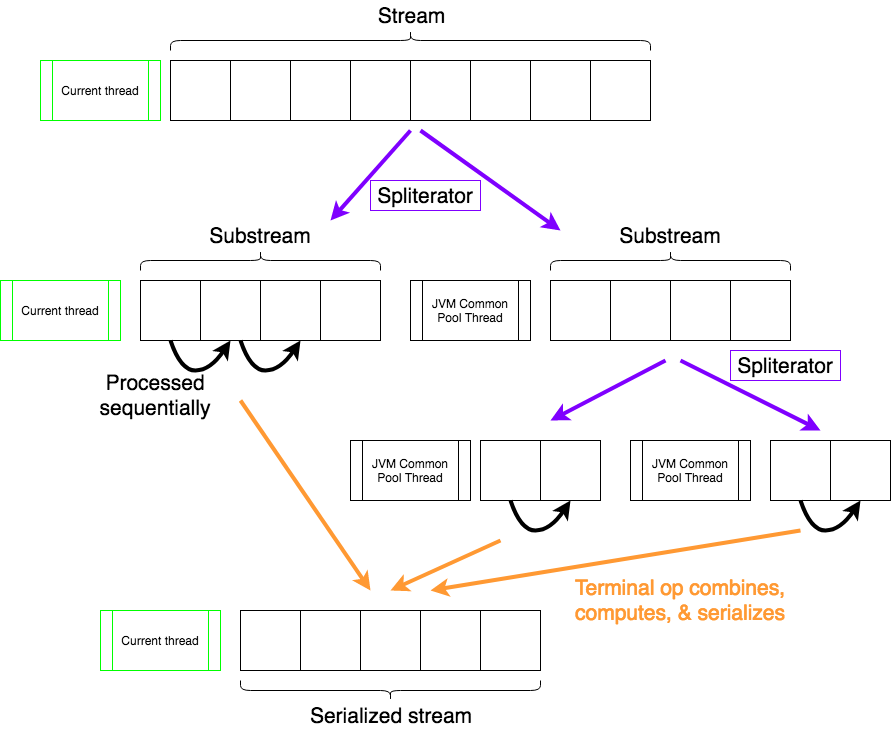
\includegraphics[width=13cm]{../images/overview.png}
\caption{Overview of a Parallel Stream}
\source{Ethan Williams}
\label{fig:overview}
\end{figure}

There are several terminal operations for a parallel stream, but the \verb|collect()| method is the most reliable form of reduction. The method uses a \verb|Collector| to reduce the stream, an object that defines how input elements should be added to a given data structure. This document will focus on the \verb|Collector|'s functionality and implementation, finishing with an explanation of special use cases for parallel streams.

Despite parallel streams being introduced into Java to simplify concurrency, developers can easily corrupt data and cause system bugs. All possible bugs in streams derive from developers not following standard concurrency practices such as using long-running or blocking operations in streams. Additionally, considerations have to be taken with streams specifically to avoid interference with the source and using stateful expressions.

\section{Spliterator}
The \verb|Spliterator| is the backbone of parallel streams, allowing the program to split a collection apart (illustrated in Figure \ref{fig:split}) and iterate through it. If a class extending a \verb|Collection| does not have a \verb|spliterator()| method returning a \verb|Spliterator| object, then Java is not able to process the collection with a parallel stream at all. Figure \ref{fig:split} shows how an instance may behave when it splits itself. It is worth noting that the splitting doesn't actually break up the collection. \verb|Spliterator|s share the collection and simply keep track of what element it is currently iterating on (index) and one more than the last element it is allowed to execute with (fence).

\begin{figure}[H]
\centering
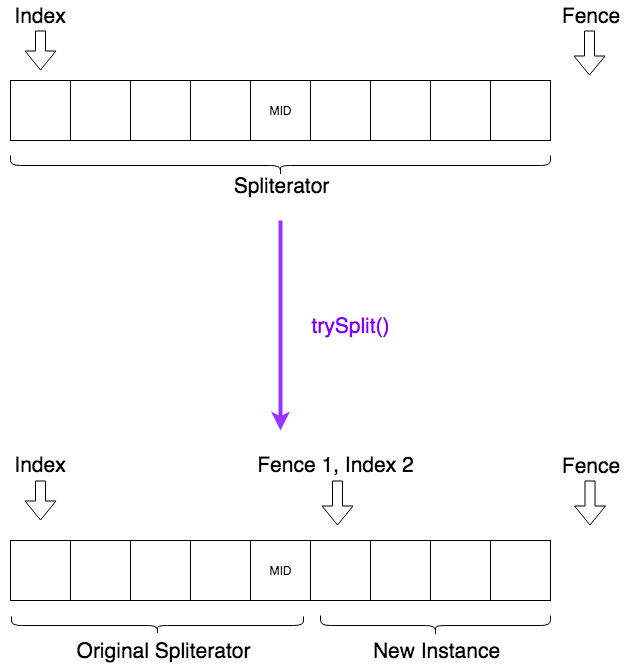
\includegraphics[width=8cm]{../images/spliterator.png}
\caption{A Spliterator Before and After Splitting}
\source{Ethan Williams}
\label{fig:split}
\end{figure}

\subsection{Implementation} 
A \verb|Spliterator| must be able to traverse and split the portion of the stream it represents. \verb|tryEachRemaining()| and \verb|tryNext()| are the two methods which dictate how traversal is handled for the collection. \verb|tryEachRemaining()| in Figure \ref{fig:forEachRemaining} takes a Consumer object which is the operation to be executed on each element of the collection. The example simply iterates through each element and uses it as a parameter to the \verb|accept()| method of the \verb|Consumer| object. \verb|tryNext()| in Figure \ref{fig:tryAdvance} is similar although the operation is only attempted on element at the current cursor position. If that cursor position is past the fence of the Spliterator, then the method returns false, otherwise it returns true.

\begin{figure}[H]
\centering
\begin{lstlisting}[language=Java]
public void forEachRemaining(Consumer<? super E> action) {
    int i;
    if ((i = index) >= 0 && (index = fence) <= a.length) {
        for (; i < hi; ++i)  action.accept((E) list.elementData[i]);
    }
    throw new ConcurrentModificationException();
}
\end{lstlisting}
\caption{Implementation of forEachRemaining()}
\source{Java ArrayList, modified by Ethan Williams}
\label{fig:forEachRemaining}
\end{figure}

\begin{figure}[H]
\centering
\begin{lstlisting}[language=Java]
public boolean tryAdvance(Consumer<? super E> action) {
    int hi = getFence(), i = index;
    if (i < hi) {
        index = i + 1;
        action.accept((E) list.elementData[i]);
        return true;
    }
    return false;
}
\end{lstlisting}
\caption{Implementation of tryAdvance()}
\source{Java ArrayList, modified by Ethan Williams}
\label{fig:tryAdvance}
\end{figure}

A \verb|Spliterator|'s primary functionality is encapsulated within the \verb|trySplit()| method in Figure \ref{fig:trySplit}. This method is called when the JVM wants to break the source collection in order to start processing the stream on another thread and if implemented incorrectly can be a subtle but important error in an application \autocite{}. The example implementation simply finds the midpoint and either returns a new \verb|Spliterator| from the cursor to the midpoint and the current instance of \verb|Spliterator| now covers mid to the fence. The example \verb|trySplit()| method is the code behind the split behavior illustrated in Figure \ref{fig:split}.

\begin{figure}[H]
\centering
\begin{lstlisting}[language=Java]
public Spliterator<E> trySplit() {
    int lo = index, mid = (lo + fence) >>> 1;
    return (lo >= mid) ? null : new Spliterator<E>(list, lo, index = mid);
}
\end{lstlisting}
\caption{Implementation of trySplit()}
\source{Java ArrayList, modified by Ethan Williams}
\label{fig:trySplit}
\end{figure}

\section{Collector}
A \verb|Collector| object defines a mutable reduction operation for a group of input elements, in other words, it provides information on how to instantiate a data structure and perform several operations on it. Its functionality is encompassed in 4 methods (illustrated in Figure \ref{fig:collector}):

\begin{itemize}
\item \verb|supplier()| provides information on how to construct a new instance of the desired data structure
\item \verb|accumulator()| details how to add any given element to the data structure
\item \verb|combine()| method simply assembles multiple instances of the data structure
\item \verb|finisher()| method simply serializes the stream, completing the reduction
\end{itemize}

\begin{figure}[H]
\centering
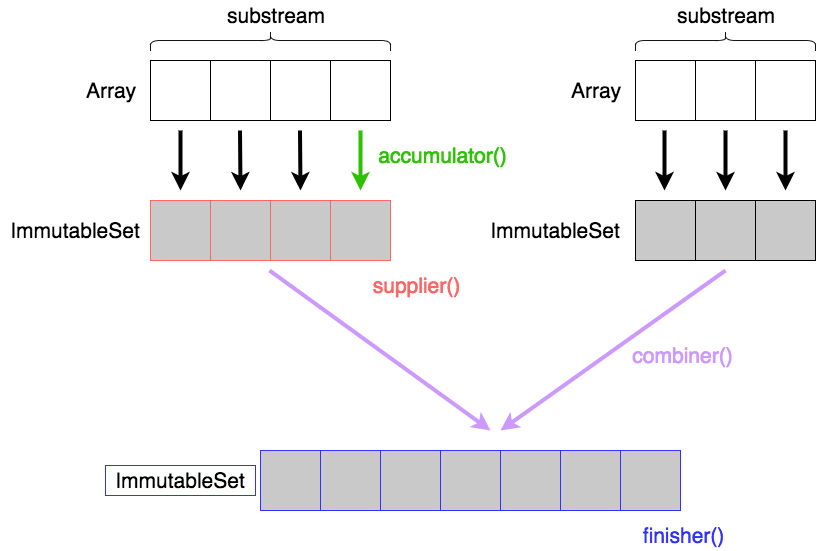
\includegraphics[width=13cm]{../images/collector.png}
\caption{How a Collector is Used}
\source{Ethan Williams}
\label{fig:collector}
\end{figure}

\verb|Collector| objects are used during a reduction operation to join substreams together in the form of the data structure defined by the instance. Java has a static class called \verb|Collectors| which provide basic reduction instances via method calls. For example \verb|Collectors.toMap()| returns a \verb|Collector| instance which reduces the stream to a \verb|Map|. 

\subsection{Implementation}

A \verb|Collector| object has four methods which comprise the majority of its functionality: \verb|supplier()|, \verb|accumulator()|, \verb|combiner()|, \& \verb|finisher()| \autocite{collector_doc}. The examples below are a \verb|Collector| which will yield an \verb|ImmutableSet| when used.

The \verb|supplier()| method returns a mechanism to build an instance of a mutable data structure that will hold the elements of the stream called an \textit{accumulator} \autocite{custom_collector}, in our code example this is a builder for \verb|ImmutableSet|.

\begin{figure}[H]
\centering
\begin{lstlisting}[language=Java]
public Supplier<ImmutableSet.Builder<T>> supplier() {
    return ImmutableSet::builder;
}
\end{lstlisting}
\caption{Implementation of supplier()}
\source{Ethan Williams}
\label{fig:supplier}
\end{figure}

The \verb|accumulator()| method takes an accumulator and an element as parameters and will return a \verb|Consumer| object which details how the element should be added to the accumulator. In the example a \verb|BiConsumer| object will add the element to the given \verb|ImmutableSet|.

\begin{figure}[H]
\centering
\begin{lstlisting}[language=Java]
public BiConsumer<ImmutableSet.Builder<T>, T> accumulator() {
    return (builder, t) -> builder.add(t);
}
\end{lstlisting}
\caption{Implementation of accumulator()}
\source{Ethan Williams}
\label{fig:accumulator}
\end{figure}

The \verb|combiner()| method details the logic on how two accumulators should be joined together and is used to assemble all instances of the new data structure that were derived from substreams. In the code example the \verb|combiner()|'s behavior is that when two \verb|ImmutableSet|s are combined, one is simply appended to the other.

\begin{figure}[H]
\centering
\begin{lstlisting}[language=Java]
public BinaryOperator<ImmutableSet.Builder<T>> combiner() {
    return (left, right) -> {
        left.addAll(right.build());
        return left;
    };
}
\end{lstlisting}
\caption{Implementation of combiner()}
\source{Ethan Williams}
\label{fig:combiner}
\end{figure}

Finally, the \verb|finisher()| method serializes the accumulator that is the result of combining all the substreams, completing the reduction. In the code example, this is as easy as returning the \verb|build()| method which serializes the \verb|ImmutableSet|, completing the conversion of the source.

\begin{figure}[H]
\centering
\begin{lstlisting}[language=Java]
public Function<ImmutableSet.Builder<T>, ImmutableSet<T>> finisher() {
    return ImmutableSet.Builder::build;
}
\end{lstlisting}
\caption{Implementation of finisher()}
\source{Ethan Williams}
\label{fig:finisher}
\end{figure}

\subsection{Special Uses for Parallelism}
Although the \verb|collect()| method can be used on both serial and parallel streams, Java also includes special \verb|Collector| instances for better parallel performance. For example, Figure \ref{fig:employee_collection} has the same collect operation on a parallel stream, one reduces with the \verb|groupingBy()| method and the other reduces with the \verb|groupingByConcurrent()| method. Even though both are parallel, the second example runs significantly faster because the reduction can be parallelized by using a \verb|ConcurrentMap|. The first example processes each element in parallel, but the reduction is to a non-thread-safe data structure, limiting the potential benefits of parallelism.

\begin{figure}[H]
\centering
\begin{lstlisting}[language=Java]
// Example 1
ConcurrentHashMap<Department, List<Employee>> byDept
    = employees.stream()
               .parallel()
               .collect(Collectors
                  .groupingBy(Employee::getDepartment)
                );
                
// Example 2
Map<Department, List<Employee>> byDept
    = employees.stream()
               .parallel()
               .collect(Collectors
                  .groupingByConcurrent(Employee::getDepartment)
                );
\end{lstlisting}
\caption{Reduction of employees into map by a Collector}
\source{Ethan Williams}
\label{fig:employee_collection}
\end{figure}

\section{Practical Considerations when Using Parallel Streams}
Parallel streams were introduced to make implementing parallelism in a Java application easier, but with this ease comes common pitfalls that arise from the abstraction. For example, a common mistake is using long-running or blocking operations in a stream which is a bad concurrency practice to begin with. Additionally, many developers aren't familiar with interference and stateful expressions which can lead to severe errors in the application.

\subsection{Long-Running/Blocking Operations}
Using long-running or blocking operations in a stream will degrade performance drastically, a result of how streams implement threading. The JVM begins by processing on the calling thread and as more subtasks are broken off, the JVM gets threads from \verb|ForkJoinPool.common()|, which is a thread pool used in the background of the whole application \autocite{dzone_dangers}. 

With the JVM's use of a common thread pool, a long-running operation in a parallel stream as shown in the first example of Figure \ref{fig:network_op} will degrade performance drastically. Performance will be such that the stream will benefit very little from parallelization and may even be less performant than a serial stream. Each thread in the pool will be consumed executing that operation and subsequently all other JVM tasks using the common thread pool have to wait. 

In a situation where several streams are all attempting to process in parallel, each stream's performance will suffer even if it should have no problem. Java does allow a custom \verb|ThreadPool| like in example 2 of Figure \ref{fig:network_op} which can help by using threads created outside the common pool \autocite{dzone_fjp}. Unfortunately, since the issue described above results from a bad concurrency practice, more threads won't provide any significant performance enhancement.

\begin{figure}[H]
\centering
\begin{lstlisting}[language=Java]
// Example 1
Optional<String> result = collection.stream().parallel().map((base) -> longOperation(argument)).findAny();

// Example 2
ForkJoinPool customPool = new ForkJoinPool(4);
Optional<String> result = customPool.submit(() -> collection.stream().parallel().map((arg) -> longOperation(arg)).findAny()).get();
\end{lstlisting}
\caption{Reduction of employees into map by a Collector}
\source{Ethan Williams}
\label{fig:network_op}
\end{figure}

\subsection{Interference}
Since \verb|Stream|s don't contain any of the elements of the collection, instead storing references, if the source is modified then the reference is invalidated \autocite{ibm_streams}. Editing the source of the stream in an intermediate operation is called \textit{interference} and will throw a \verb|ConcurrentModificationException| \autocite{parallelism_doc}. The stream in figure \ref{fig:interference} attempts to add each element to the collection again using the \verb|map()| method. Since it attempts to modify the source before the stream has serialized, this operation will throw an exception.

\begin{figure}[H]
\centering
\begin{lstlisting}[language=Java]
collection.stream().parallel().map((x) -> collection.add(x)).toArray();
\end{lstlisting}
\caption{A stream which causes interference and will throw an error}
\source{Ethan Williams}
\label{fig:interference}
\end{figure}

\subsection{Stateful Expressions} \label{stateful_expressions}
The third practice which will cause errors in a stream and should be watched carefully is using stateful expressions, which are operations that depends on the ordering of the elements \autocite{expression_state}. The code in Figure \ref{fig:stateful} shows an example of a stateful operation while attempting to add elements to \verb|parallelStorage| and print them. Although the \verb|forEachOrdered()| method is just fine and will print in the expected order, \verb|parallelStorage| will have a different ordering every time the stream is executed. The addition is stateful, meaning it depends on ordering and in parallel streams ordering can't be guaranteed in intermediate operations \autocite{parallelism_doc}.

\begin{figure}[H]
\centering
\begin{lstlisting}[language=Java]
List<String> parallelStorage = Collections.synchronizedList(new ArrayList<>());
collection.stream().parallel().map(x -> parallelSotrage.add(x)).forEachOrdered(x -> System.out.println(x));
\end{lstlisting}
\caption{A stream which causes interference and will throw an error}
\source{Ethan Williams}
\label{fig:stateful}
\end{figure}
 
\printbibliography[heading=bibintoc]

\end{document}